\documentclass[DIV=calc, paper=a4, fontsize=11pt, twocolumn]{scrartcl}
\usepackage[titletoc,toc]{appendix}
%\usepackage[french]{babel}
\usepackage[utf8]{inputenc}
\usepackage[T1]{fontenc}
\usepackage{hyperref}
\hypersetup{
    colorlinks,
    linkcolor={red!50!black},
    citecolor={blue!50!black},
    urlcolor={blue!80!black}
}
\usepackage{amssymb}
\usepackage{graphicx}
\usepackage[protrusion=true,expansion=true]{microtype} 
\usepackage{amsmath,amsfonts,amsthm} 
\usepackage[svgnames]{xcolor} 
\usepackage[hang, small,labelfont=bf,up,textfont=it,up]{caption} 
\usepackage{fix-cm}	 % Custom font sizes - used for the initial letter in the document
\usepackage{subcaption}
\usepackage{sectsty} 
\allsectionsfont{\usefont{OT1}{phv}{b}{n}} 
\usepackage{fancyhdr} 
\pagestyle{fancy} 
\usepackage{lastpage} 

\lhead{}
\chead{}
\rhead{}

% Footers
\lfoot{}
\cfoot{}
\rfoot{\footnotesize Page \thepage\ of \pageref{LastPage}} % "Page 1 of 2"

\renewcommand{\headrulewidth}{0.0pt}
\renewcommand{\footrulewidth}{0.4pt}

\usepackage{lettrine} 
\newcommand{\initial}[1]{ 
\lettrine[lines=3,lhang=0.3,nindent=0em]{
\color{DarkGoldenrod}
{\textsf{#1}}}{}}

\usepackage{titling} % Allows custom title configuration

\newcommand{\HorRule}{\color{DarkGoldenrod} \rule{\linewidth}{1pt}} 

\pretitle{\vspace{-30pt} \begin{flushleft} \HorRule \fontsize{40}{40} \usefont{OT1}{phv}{b}{n} \color{DarkRed} \selectfont} % Horizontal rule before the title

\title{ A Machine Learning Score for non listed Companies Based on Balance Sheets}

\posttitle{\par\end{flushleft}\vskip 0.5em} % Whitespace under the title

\preauthor{\begin{flushleft}\large \lineskip 0.5em \usefont{OT1}{phv}{b}{sl} \color{DarkRed}} % Author font configuration

\author{Juan Barragan} 

\postauthor{\footnotesize \usefont{OT1}{phv}{m}{sl} \color{Black} % Configuration for the institution name

Kommets.com % Your institution

\par\end{flushleft}\HorRule} % Horizontal rule after the title

\date{} 

%----------------------------------------------------------------------------------------

\begin{document}
\maketitle 
\tableofcontents
\thispagestyle{fancy}
\begin{abstract}
\section{Introduction}
According to the  Banks Federation (Fédération des Banques Françaises) The amount of loans given to Non Listed Small Caps 
over one year (from July 2015 to July 2016) in France stands at 385,2 billions Euros. And that liquidity helps to finance more than 
one million businesses. One of the challenges for giving credit to non listed companies is to assess their credit risk. 
On this paper we propose a \emph{scoring model} for measuring the \emph{Default Risk} using preceding balance sheets.

We are going to use big data techniques, namely \emph{Machine Learning} for selecting key financial indicators allowing to predict default.
We synthesize these indicators on a unique number, the \emph{score}. This score is going to reflect, for a given enterprise, the default 
risk. In addition, the score combined with a zero coupon curve for a given country can be easily correlated to a rate of return for loans. 

\end{abstract}
%----------------------------------------------------------------------------------------
%	ARTICLE CONTENTS
%----------------------------------------------------------------------------------------

\section{The data set}
The French central bank have a data set of French enterprises, but this data base is not generally available \footnote{This has changed as of July 2017.
French government has release through the INPI a data set of balance sheets. But this includes only one year of historical data, not enough 
for building a model}. 
In looking for data-sets, we have found that the Central Bank of Belgium through the 
\href{https://www.nbb.be/fr/centrale-des-bilans}{Balance Sheet Center} has a complete data-set with several decades of
historical data.

\subsection{Description of the Enterprises}
Among all the balance sheets, we have selected the enterprises which are appropriate for a financial study. These are:
\begin{itemize}
    \item European Cooperative Society
    \item Cooperative Society with Unlimited Liability
    \item Cooperative Society with Limited Liability
    \item Participating Cooperative Society with Limited Liability
    \item Private Limited Company
    \item Partnership Company
    \item Partnership Company by Actions
\end{itemize}
To these societies, we consider the status Either the society is in normal situation, either she is in default:
\begin{itemize}
    \item Default (Declaration, opening)
    \item Default ended excusably.
    \item Default ended non excusably.
\end{itemize}
This will allow us to analyze the societies with healthy status or with real default. We avoid enterprises who disappear by fusion, or
wanted dissolution, scission, etc.
Still among that subset we want to concentrate our attention to small and medium enterprises, these are societies whose size:
\begin{itemize}
    \item Have less than 250 employees,
    \item Either annual earning are less than 50 millions Euros, either their balance sheet is less than $40$ millions euro's. And for avoiding very small enterprise, which are really fragile,
    \item We excluded enterprises whose number of employees is less than or equal 40.
\end{itemize}

\section{Tools}
\subsection{Software Tools}
For realizing this note, we have used techniques from \emph{Machine Learning}, through software tools as \href{https://www.python.org/}{python}
and \href{http://scikit-learn.org/stable/}{scikit}.  A parallel computing engine \href{http://spark.apache.org/}{Spark}. The
date we have analyzed is nos structured neither fixed in size so we choose a NoSQL data base \href{https://www.mongodb.com/}{mongo}.

Machine Learning is a branch with origins in Engineering and Computer Science which focuses in finding patters for classification using 
tools from Statics, Analysis and Geometry.
Machine Learning will be very nicely adapted for us. We are going to explore several millions of accounting data looking
for patterns allowing us to predict default given evidence in the balance sheet.
This is made usually by financial analysts by hand with empirical criteria for determining critical thresholds.
Our goal here is to formalize these methodologies by finding precise critical thresholds.


\subsection{Principal Component Analysis}
\emph{Principal Component Analysis} is a Statistical methodology allowing us to transform
a collection of vectors $X_1, X_2, \ldots X_k$, $X_i \in \mathbb{R}^n$ on another collection
$Y_1, Y_2, \ldots Y_k$ $Y_i \in \mathbb{R}^m$, with $m \leq n$ and zero correlation among them.
Vectors $Y_i$ are called \emph{Principal Components}. The fact their dimension can be lowered keeping the variance is of great help whenever we look for visualizing a big number of observables.

Technically we can calculate these variables as follows, let $\mathbf{m}$ 
be the mean vector, $\mathbf{m} = 1/k\sum_{i=1}^k X_i$, let $\mathbf{S}$ and  
$\mathbf{S} = 1/k \sum_{i=1}^k (X_i - \mathbf{m})(X_i - \mathbf{m})^t$, the co-variance matrix, $X^t$ being the transpose.
  of $X$. For reducing an $m$ dimensional space is enough to calculate the $m$ eingenvectors of $\mathbf{S}$ $v_1, \ldots v_m$, having the biggest eigenvalues. 
let $\mathbf{W} = (v_1, \ldots v_m)$, be matrix of dimension $n \times m$. The space we are looking for $Y$, is given by $Y = \mathbf{W}^t X$.
\subsection{K-Means Lloyd algorithm}
$K-$Means is an algorithm for finding aggregates on unlabeled data-sets. More precisely, given $m$ values $X_1, X_2, \ldots X_m$ and $k$ an integer, we look for a partition of the values into $k$ classes, $S_1, S_2,\ldots, S_k$  and their centers $c_1, c_2, \ldots c_k$ such that
$$\sum_{i = 1} \sum_{X \in S_i} \| X-c_i\|$$
be a minimum. This can be done with the Lloyd algorithm:
\begin{itemize}
  \item[0] Pick arbitrary different centers $c_1^0, c_2^0, \ldots c_k^0$.
  \item[1] Define       
    $$S_i^n = \{ X : \| X - c_i^n \| \leq \|X - c_j^n \| \quad \forall i \neq j \}$$
  \item[2] Then the new centers are
    $$c_i^{n+1} = \frac{1}{|S_i|} \sum_{X \in S_i} X$$
with $|S_i|$ the cardinality of $S_i$.
  \item[3] repeat steps $1$ and $2$ until a given tolerance threshold.
\end{itemize}
\begin{figure}
  \centering
    
\includegraphics[width=0.5\linewidth]{centers}
  \caption{$K$-Means classes}
  \label{fig:kmeans}
\end{figure}
See \ref{fig:kmeans} for a $K-$means example.
\subsection{Logistic Regression}
Let again $X_1, X_2, \ldots X_k$, $X_i \in \mathbb{R}^n$ be a set of points and $\lambda : \mathbb{R}^n \to \{0,1\}$ a \emph{labeling system}. Let $Y_i = \lambda(X_i)$, we can consider $Y$ as a Bernoulli Random Variable. Given a value $X_0$, we write the probabilities:
$$\mathbb{P}(Y=1| X = X_0) = p,$$
$$\mathbb{P}(Y=0| X = X_0) = 1-p$$
or more compactly:
\begin{equation}
\mathbb{P}(Y=Y_0| X = X_0) = p^{Y_0}(1-p)^{1-Y_0}.
\label{eqn:bern}
\end{equation}
We have here a classification problem, If the labeling is separable, there exist an hyper-plan $L: \mathbb{R}^n \to \mathbb{R}$, $L_{\theta, \theta_0}(X) = \theta X + \theta_0$ such that
$$ L_{\theta, \theta_0}(X_i) > 0, \quad \text{if} \quad Y_i = 1, \quad \text{and}$$
$$ L_{\theta, \theta_0}(X_i) < 0, \quad \text{if} \quad Y_i = 0.$$
Using the distance to the separating hyper-plan we can smooth the probability of the Bernoulli random variable using the \emph{sigmoid} function, $s(x) = 1/(1+ e^{-x})$. For this is enough to write for each observation $X_i$, 
\begin{align*}
p &= \mathbb{P}(Y=1|X_i)\\
                    &= \frac{1}{1+ e^{-L_{\theta, \theta_0}(X_i)}}\\
\end{align*}
So the Bernoulli random variable  \ref{eqn:bern} can be written as
%\begin{align*}
$$\left( \frac{1}{1 + e^{-L_{\theta, \theta_0}(X_i) }} \right)^{Y_i} \left ( 1- \frac{1}{1 + e^{-L_{\theta, \theta_0}(X_i) }} \right)^{1 - Y_i} $$
%\end{align*}
or 
$$\frac{e^{-L_{\theta, \theta_0} (X_i)^{1-Y_i}}}{1 + e^{-L_{\theta, \theta_0}(X_i)}}$$
Now, for finding the optimal parameters, $\theta, \theta_0$, we maximize the \emph{log-likelihood} over all the observations:
$$\textbf{argmax}_{\theta, \theta_0}\log \prod_{i=1}^k \frac{e^{-L_{\theta, \theta_0} (X_i)^{1-Y_i}}}{1 + e^{-L_{\theta, \theta_0}(X_i)}}$$
\begin{figure}
  \centering
    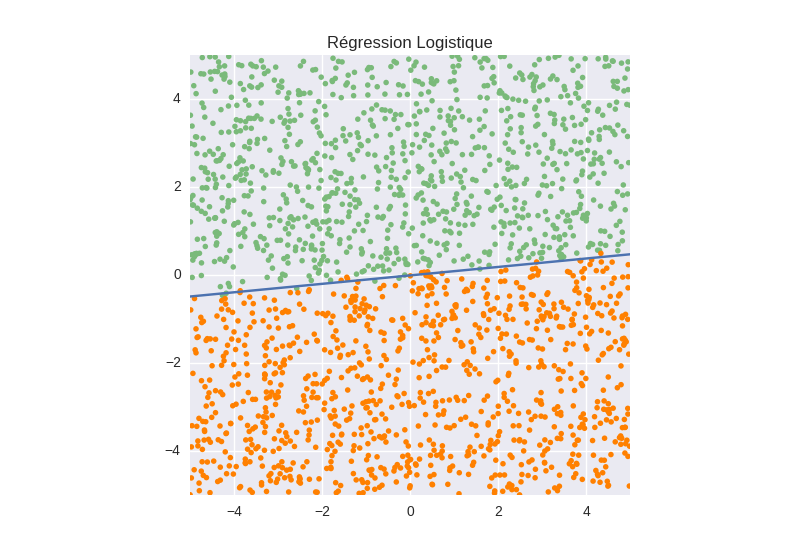
\includegraphics[width=\linewidth]{reglog}
  \caption{Logistic Regression}
  \label{fig:reglog}
\end{figure}
Figure \ref{fig:reglog} shows an example of Logistic Regression and its separating plane.
\subsection{Support Vector Machines (SVM)}
A similar methodology is provided by the \emph{Support Vector Machines}. Suppose we are exactly on the same situation than the preceding section, with a set of observations $X_1, X_2, \ldots X_k$, $X_i \in \mathbb{R}^n$. But now we change slightly our labels $\lambda : \mathbb{R}^n \to \{1, -1\}$. If a separating plane does exists, $L: \mathbb{R}^n \to \mathbb{R}$, $L_{\theta, \theta_0}(X) = \theta X + \theta_0$ such that $\textrm{sign}(L_{\theta, \theta_0}(X_i)) = \lambda(X_i)$, then we have for all $i$
\begin{equation}
\frac{\lambda_i(X_i)L(X_i)}{\|\theta\|}>0
\label{eqn:dist}
\end{equation}
We recognize on equation \ref{eqn:dist} the distance from point  $X_i$ to the hyper-plan $L_{\theta, \theta_0}$. The support Vector Machine looks for maximizing:
\begin{equation}
\textbf{argmax}_{\theta, \theta_0} \left\{ \frac{1}{\|\theta\|} \textbf{min}_i\lambda(X_i)L_{\theta, \theta_i}(X_i)\right\}
\label{eqn:svm}
\end{equation}
In order to simplify \ref{eqn:svm}, we change the scale of the plan as $\theta \to \kappa \theta$ and $\theta_0 \to \kappa \theta_0$ so that if $X_p$ is the point realizing the minimum $\textbf{min}_i\lambda(X_i)L_{\theta, \theta_i}(X_i)$, then for that point $X_p$ we have $\lambda(X_p)L_{\theta, \theta_0}(X_p) = 1$. Hence the optimization program \ref{eqn:svm} can be written:
$$\textbf{argmax}_{\theta, \theta_0}  \frac{1}{\|\theta\|}, \quad i = 1, \dots k$$
or equivalently: 
$$\textbf{argmin}_{\theta, \theta_0}  \frac{1}{2}\|\theta\|^2, \quad i = 1, \dots k$$
with the constraints
$$ \lambda(X_i)L_{\theta, \theta_0}(X_i) \geq 1 \quad i = 1, \ldots k$$
\begin{figure}
  \centering
    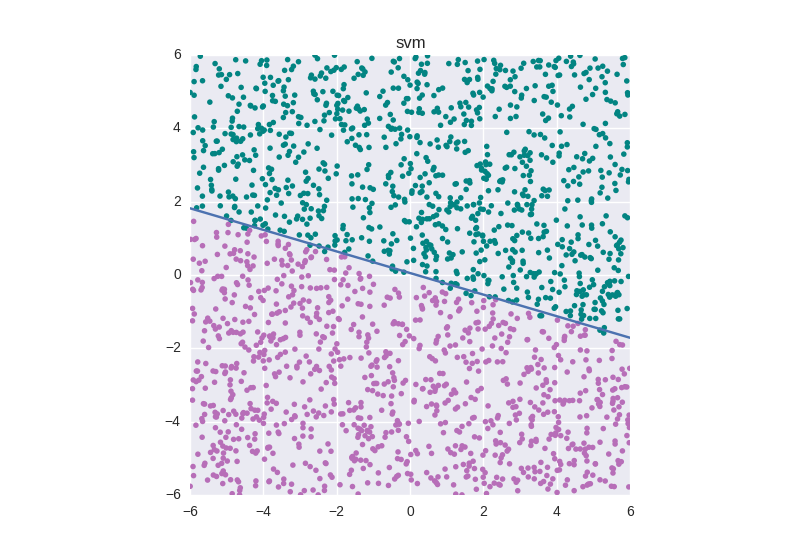
\includegraphics[width=\linewidth]{svm}
  \caption{Support Vector Machine}
  \label{fig:svm}
\end{figure}
Figure \ref{fig:svm} shows an example of separating plane calculated with support vector machines.

\section{Analysis of Financial Ratios}
Creditworthiness analysis is realized by looking at financial ratios on the balance sheet, experts select the ones being relevant 
for financial health.

A pioneer in doing scoring is Altman see  \cite{Altman}. For detecting when an enterprise is near default,
the author proposes a criteria using discriminant on financial ratios. 
Altman's discriminant is an hyper-plan $Z = V_1X_1 + V_2X_2 + \ldots V_nX_n$, where $V_i$ are the discriminant coefficients
and $X_i$ the independent variables coming from balance sheet financial ratios. 
Altman score is directly linked to the creditworthiness of the enterprise, the actual hyper-plan found by Altman is
\begin{align*}
Z =& \enskip 0.012X_1  + 0.014X_2 + \\
  & \enskip 0.033X_3 +   0.006X_4 +  0.999X_5\\
\end{align*}
with 
\begin{itemize}
  \item[] $X_1$ Working capital over total assets. This measures liquid assets in relation to the size of the company.
  \item[] $X_2$ Retained earnings over total assets. Which measures profitability. 
  \item[] $X_3$ EBDITA over total assets. EBDITA being earnings before interest and taxes, which measures operating efficiency apart from tax.
  \item[] $X_4$ Market value of equity over book value of liabilities
  \item[] $X_5$ Sales over total assets.
\end{itemize}
Altman found that the ratio profile for the bankrupt group fell at $-0.25$ in average, and for the non-bankrupt
 group at $+4.48$ in average.
Our aim is to generalize this discriminant hyper-plane using Machine Learning, we are going notably to use Support Vector Machines (SVM) 
and Logistic regressions for estimating the coefficients.

\subsection{Ratios of Belgium Central Bank}
The number of ratios we are going to use are $21$ and they are calculated by the Belgium Central Bank. A presentation of these ratios can be 
found on the site \href{https://www.nbb.be/fr/centrale-des-bilans}{Centrale des Bilans}

Altman's method cannot be used here as most Small Caps are not trade publicly.
Our sample of Belgian Small Caps which have a balance sheet not exceeding 40 million Euros and with at least 40 employees is of size $4796$. 
Among these 45 did default, 22 on year 2015, 22 on year 2014 an one in year 2013.

We remark an immediate difficulty here, defaults are rare, we have less than $1\%$. Another difficulty can be
appreciated using Principal Component Analysis on the ratios of year 2013. See figure \ref{fig:pca2D}, defaulted enterprises on 2014 (in red) 
are really scattered.
We can illustrate the difficulties of being rare and scattered using naively Machine Learning tools to that sample.
So using the 2013 ratios and separating enterprises healthy on 2014 and in default on 2014, we use logistic regression
\ref{fig:elog} and support vector machines \ref{fig:esvm} projected on two dimensional plan.

\begin{figure}
  \centering
    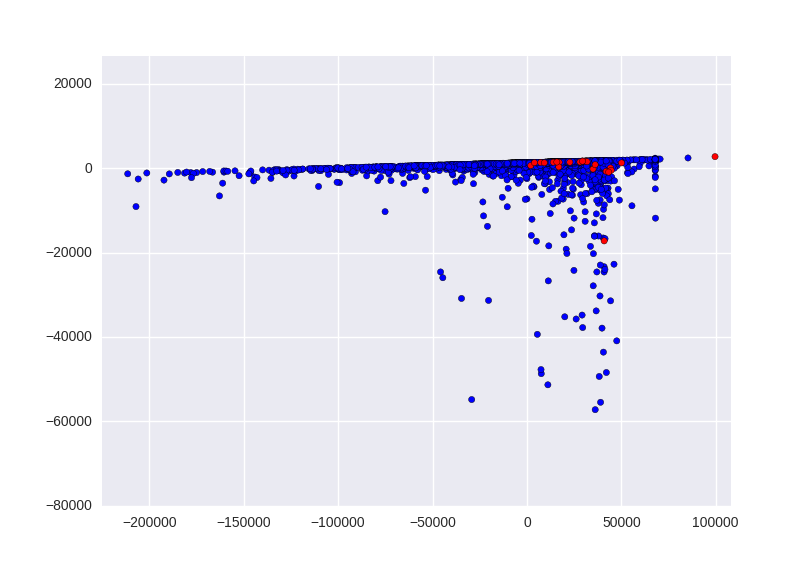
\includegraphics[width=\linewidth]{pca2D}
  \caption{PCA 2D, ratios 2014}
  \label{fig:pca2D}
\end{figure}
\begin{figure}
  \centering
    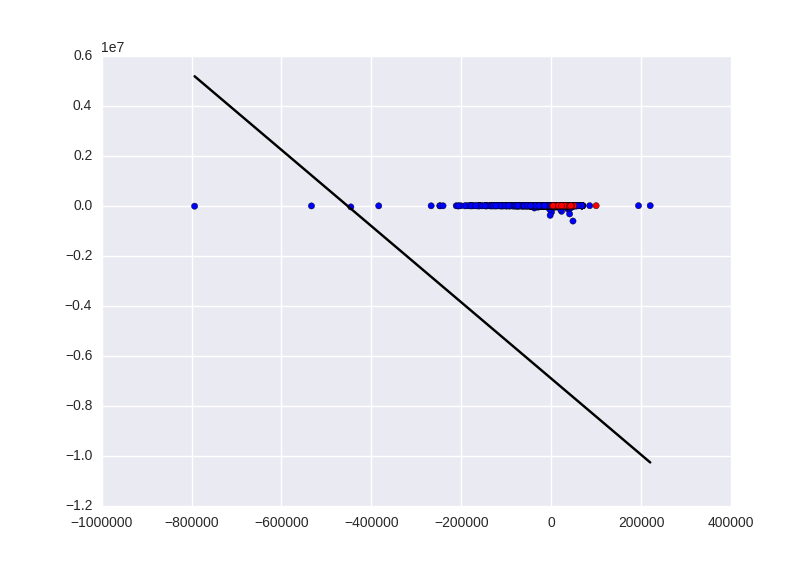
\includegraphics[width=\linewidth]{elog}
  \caption{Logistic Regression}
  \label{fig:elog}
\end{figure}
\begin{figure}
  \centering
    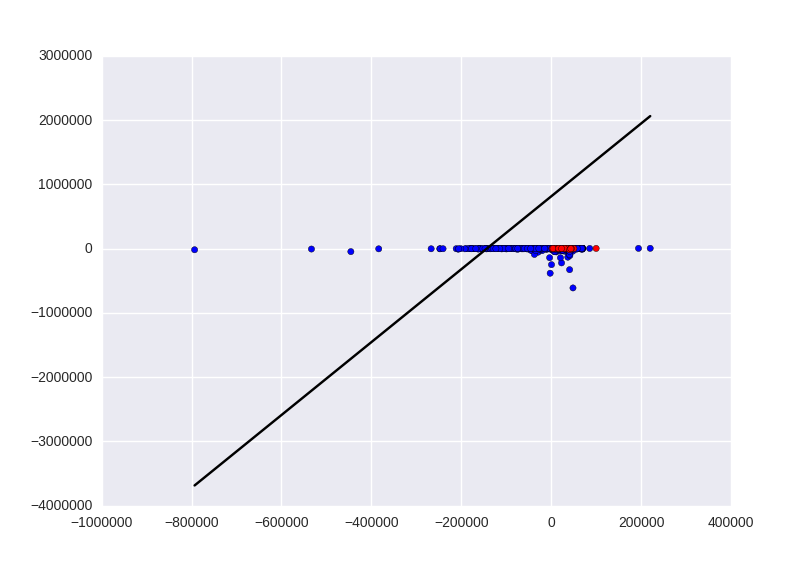
\includegraphics[width=\linewidth]{esvm}
  \caption{Support Vector Machine}
  \label{fig:esvm}
\end{figure}

As we can see results are mediocre, no method can separate the ratios.

\subsection{Selecting a better sample}
Inspired by the methodology of Altman we want to get ride of the seen difficulties by restricting our attention to a better sample.
We take the whole defaulted enterprises on 2014 and working with 2013 ratios, we are going to better select the healthy ones. 
Let $\mathcal{E}$ be the set of all enterprises, $\mathcal{S}$ the healthy ones and $\mathcal{D}$ those being on default on 2014. 
Associated to each enterprise $e$ there exists a set of ratios $r_i(e)$. Let
$$R_i = \max \{ r_i(e) | e \in \mathcal{D} \},$$
$$E_i = \{ e \in \mathcal{S} : r_i(e) \geq R_i \}$$
We look for a subset of ratios, $r_i$ such that $\cap E_i \neq \varnothing$ and such that the cardinality be comparable to the 
enterprises on default
$\#\cap E_i \sim \#\mathcal{D}$. 

Using \href{http://spark.apache.org/}{Spark} we have calculated all the intersections. Additionally, for helping our
analysis, we have done bidimentional scatterplots and histograms for selecting the best discriminants, (See appendix C)
For a concrete example, we have selected defaulted enterprises on 2014 and we have selected healthy enterprises with the following best 2013 ratios:
\begin{itemize}
\item Net margin over sales
\item Added value by employee, 
\item Liquidity  (Treasury, accounts payable, available values, value of stocks)
\item Capital over total asset.
\end{itemize}
We have found there are 29 healthy enterprises. Applying logistic regression and realizing a contour plot representing the probability 
of survival, all projected on two dimensions using principal components.
See figure \ref{fig:reglogsample}. This is very encouraging.

\begin{figure}
  \centering
    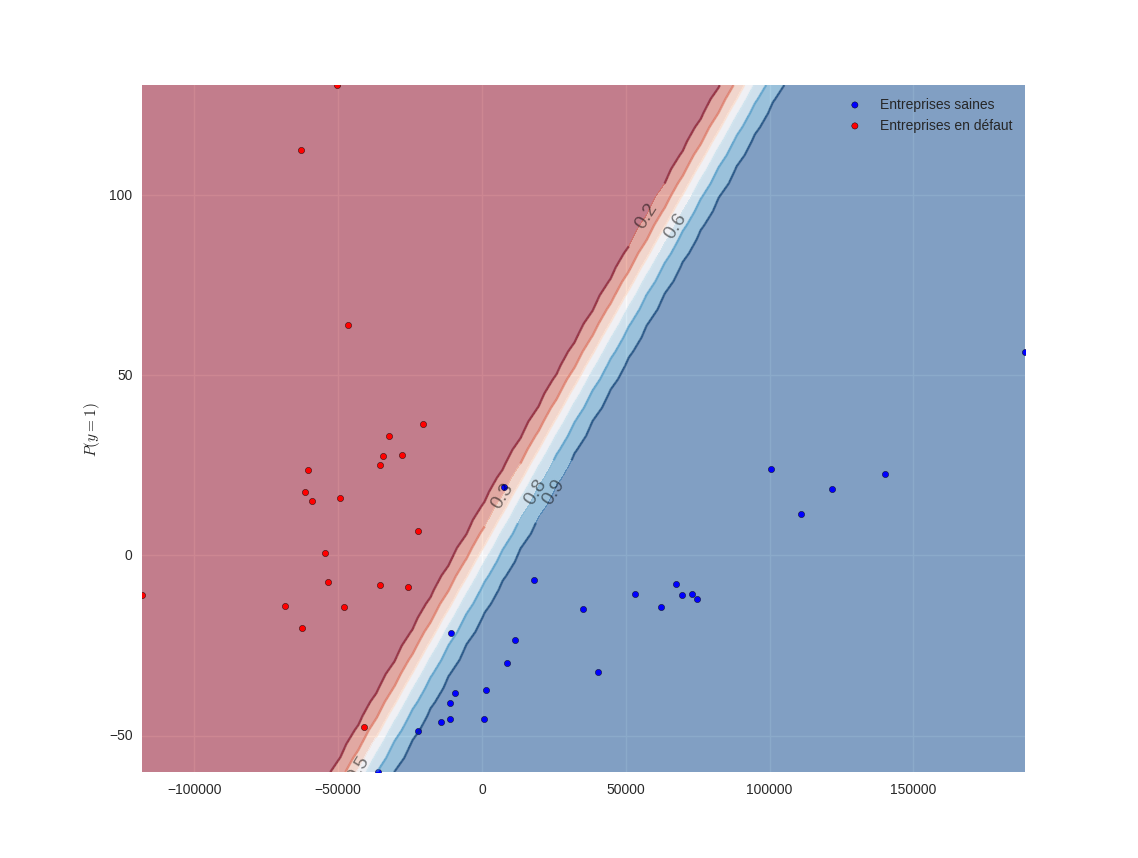
\includegraphics[width=\linewidth]{reglogsample}
  \caption{Logistic Regression and Survival Probability}
  \label{fig:reglogsample}
\end{figure}

\section{Scoring}
Now, we would like to explore all smalls data set, and for doing so we  we would like to extend the logistic regression to all 
enterprises.  
We want a \emph{Score} $R= R(e)$, such that if $\mathbb{P}_t(e|r) = \mathbb{P}_t(e| r_i, i=1, \dots n)$ 
is the survival probability on future year $t$ of the enterprise $e$ given its actual ratios $r = r_1, \ldots r_n$, then
$R$ should be that if
$$R(e_1) \leq R(e_2)$$
then 
$$\mathbb{P}_t(e_1| r) \leq \mathbb{P}_t(e_2| r)$$
In words: a better score means a better probability of survival.

Given a classificator in Machine Learning we traditionally measure its classification error. Usually, good classificators 
made less than $5\%$ errors. But this measure is meaningless for us. Defaulted enterprises on a year are less than $0.5\%$. 
A dumb classification putting every enterprise as healthy will made only $0.5\%$ errors.

So better than simple percentage of error, we are interested on what is called the \emph{True Positives} and \emph{False Positives} namely:
\begin{itemize}
\item[] True Positives (TP), which are healthy enterprises well classified,
\item[] False Positives (FP), which are defaulted enterprises well classified.
\end{itemize}
A way of synthesizing this concept is a \emph{Receiver Operating Characteristic}, ROC curve. Let us suppose we have a score $R = r(e)$ ans say
that the \emph{default threshold} is $R_0$. Meaning if $R(e) \le R_0$ then enterprise $e$ will default next year. Then the ROC curve is the 
parametric curve
$$R_0 \to (FPR(R_0), TPR(R_0)$$
Where $TPR(R_0$ is the \emph{True Positive Ratio} (True Positives over All Positives) and $FPR(R_0)$ is the \emph{False Positive Ratio} 
(False Positives over all Negatives). A cautious investor is more concerned by the False Positive Rate as it measures how well bad 
enterprises are detected.
Let $E$, be the set of all enterprises and $R =R(e)$, a score. Associate to this score the distribution function
$$F_R(x) = \frac{1}{|E|} | \{ e \in E | R(e) \leq x \} | $$
Our metric $M$ for looking for a good score assigns to the set of all defaulted enterprises $D$ a low number
$$M = 1 - \frac{1}{|D|} \sum_{e \in D} F_R(e)$$

\subsection{Natural Score}
Our Score is inspired by Altman. Consider the plane obtained by logistic regression:
$$L_{\theta, \theta_0}(X) = \sum_{i=1} \theta_i X_i + \theta_0$$
This plan separates good enterprises form bad ones. The distance from a point to this plan is given by
$$d(X, L_{\theta, \theta_0}) = \frac{L_{\theta, \theta_0}(X)}{\| \theta \|}$$
This distance is hence a good indicator of the proximity of a given enterprise to the risk zone.

So if $r_1, \ldots r_n$ are the ratios of the enterprise, our score is defined by:
$$R(e) = \sum_{i=1}^n \theta_i r_i$$
with $\theta = (\theta_1, \ldots, \theta_n)$ the discriminant coefficients of the logistic regression.
We have 21 discriminant (ratios) resulting in $2^{21} = 2 097 152$ possible combinations. Certainly there are correlations 
among the ratios. In order to reduce the number of ratios we are going to use our preceding metric $M$ on the selected intersections.
Again this is a parallel calculus done using Spark. We have around 3400 non empty intersections.

\subsection{Results}
Our best metric comes out to be obtained using the following ratios for selecting healthy enterprises, we get $3$:
\begin{itemize}
    \item Added value by employee
    \item Debt cost under Added Value
    \item Rotation of Inventories and work in progress 
\end{itemize}
Using these ratios we select a hand-full of enterprises. Applying logistic regressions tho the whole combination of ratios, we discover the following best discriminants:
\begin{itemize} %r3,r8,r10,r11,r19
  \item Added value by employee
  \item net Profit of net equity after taxes.
  \item Gross profit of total assets before taxes and financial expenses.
  \item Net profit of total assets before taxes and financial expenses.
  \item Acquisition of tangible assets over Added Value.
\end{itemize}
For these discriminants, the coefficients of the logistic regression are:
\begin{multline}
HS(X) = 0.000026X_1+0.0035X_2+0.0507X_3\\
-0.0248X_4 + 0.084X_5
\end{multline}
And we remark something interesting and surprising: the fourth ratio, Net profit of total assets before taxes and financial expenses, has a \emph{negative, impact}.
We resume the results with two graphs of ROC curves. The first one, see figure \ref{fig:roc_2014}
\begin{figure}
  \centering
    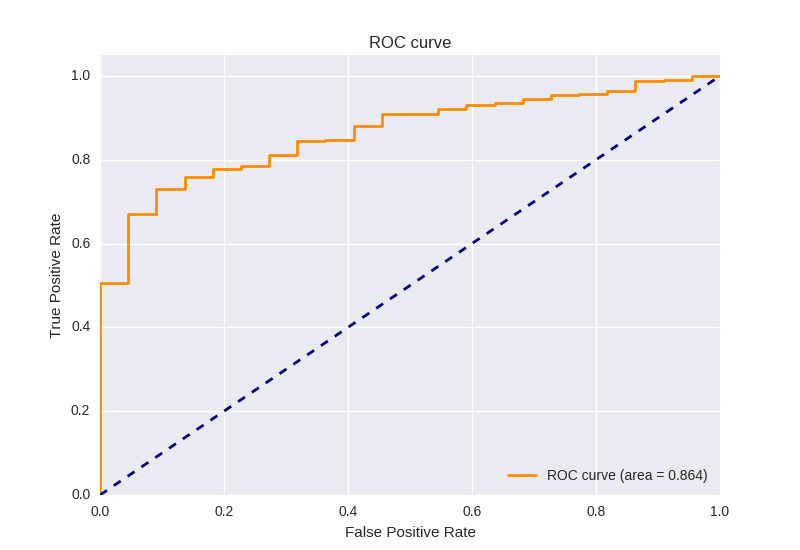
\includegraphics[width=\linewidth]{roc_2014}
  \caption{Quality of classifications for 2014}
  \label{fig:roc_2014}
\end{figure}
shows the quality of the classifier on 2014, the learned data. And the second one, see \ref{fig:roc_2015}
\begin{figure}
  \centering
    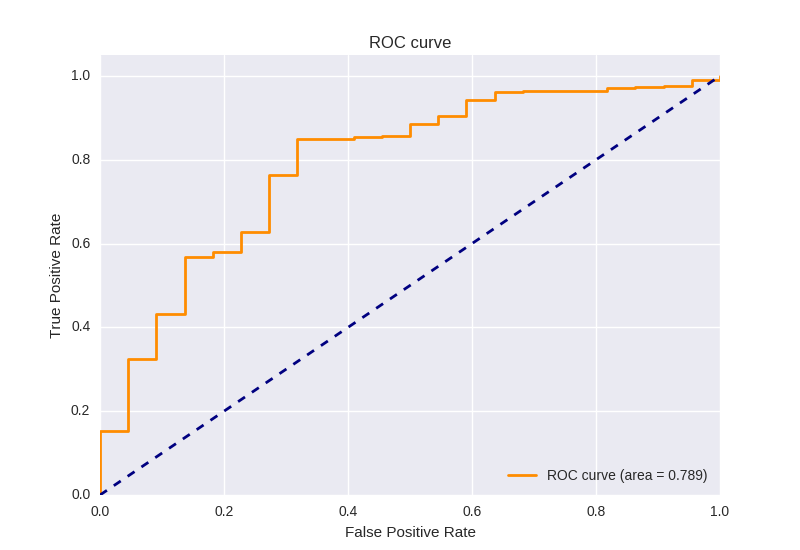
\includegraphics[width=\linewidth]{roc_2015}
  \caption{Predictive quality of classificator for 2015}
  \label{fig:roc_2015}
\end{figure}
measures the quality of the classifier for predicting outcomes on 2015, our test data. With the \emph{Area Under ROC Curve} at around $80\%$ our classifier looks as a good one. As an illustration, lets say we place our threshold for default at the score $2.50$. Then False Positive Rate is around $18\%$ and True Positive Rate is at $58\%$, look at the point $(0.18, 0,58)$ in figure \ref{fig:roc_2015}. This means that for this threshold, we neglected $100\% - 58\% = 42\%$ of healthy enterprises. But on the other hand, we only have $18\%$ chances of selecting enterprises who are going to default.
\begin{appendices}

%\onecolumn
\clearpage
\section{Histograms}
We show aggregation of ratios for the year 2014. This is a first look into distributions of the ratios. On the height axis we plot density, 
and on the horizontal axis we have plot the ratio values of the defaulted enterprises.
We ideally look for discriminants capturing on a given region all the defaulted enterprises. A good example can be see on fig , added value by employee. In this case, ahead of perhaps one outlier all red points are to the left of the histogram.
\begin{figure}[h]
  \centering
    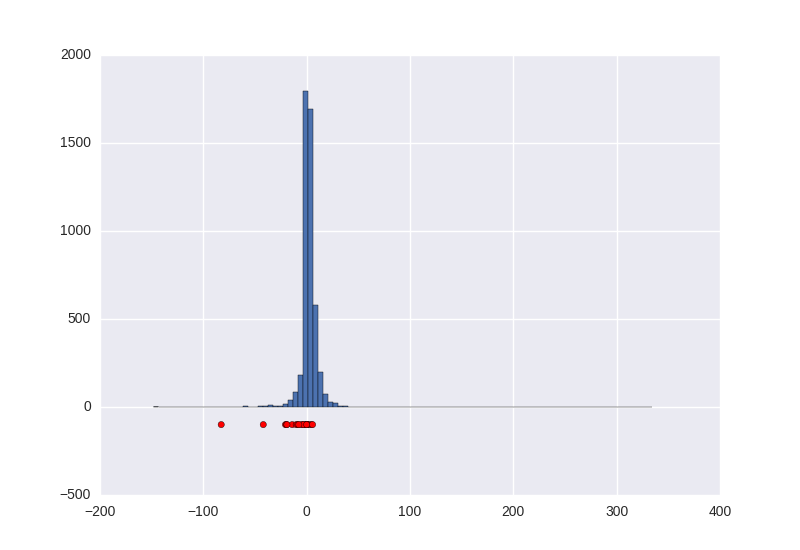
\includegraphics[width=0.8\linewidth]{r2}
  \caption{Net margin over sales}
\end{figure}
\begin{figure}[h]
  \centering
  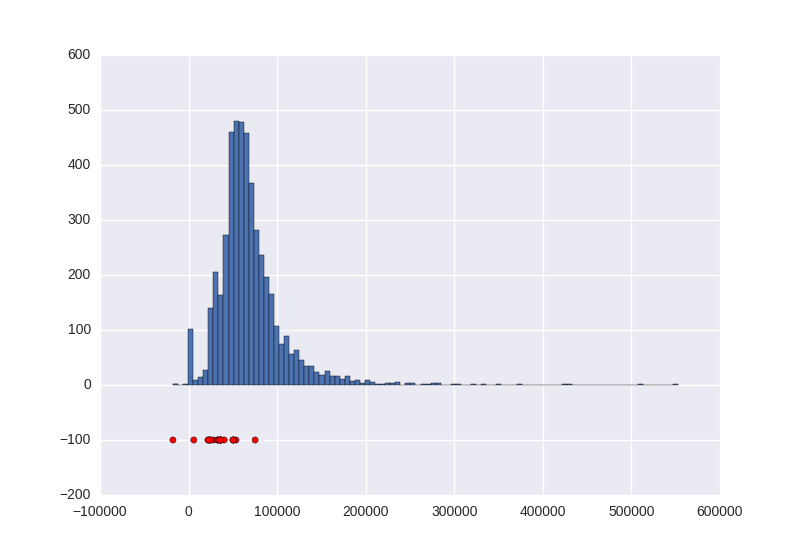
\includegraphics[width=0.8\linewidth]{r4}
  \caption{Added value by employee}
\end{figure}
\begin{figure}[h]
  \centering
  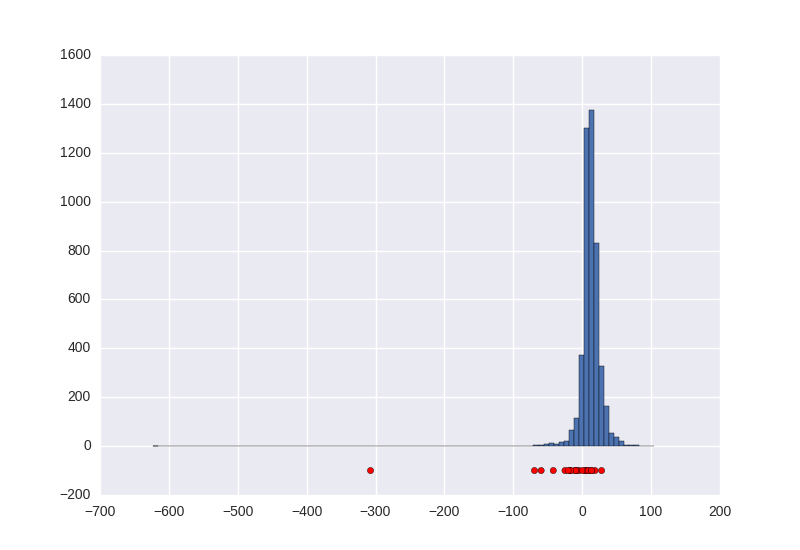
\includegraphics[width=0.8\linewidth]{r11}
  \caption{Gross profit of net equity before taxes}
\end{figure}
\begin{figure}[h]
  \centering
  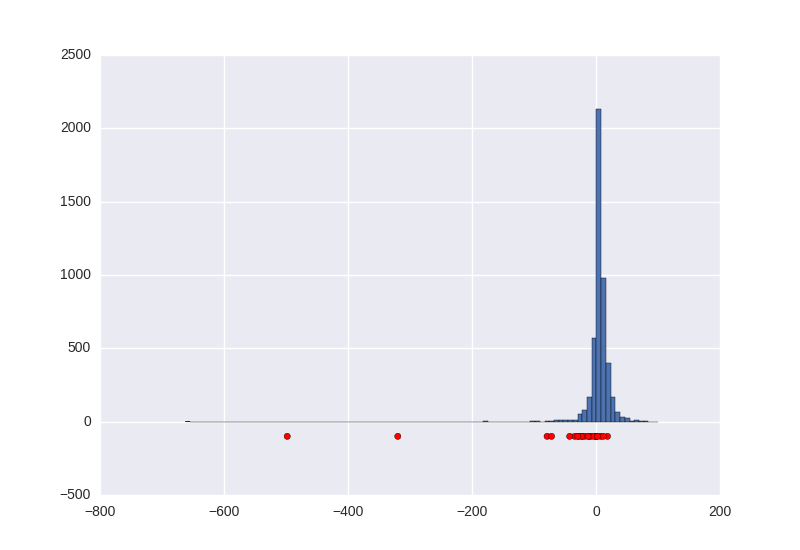
\includegraphics[width=0.8\linewidth]{r12}
  \caption{Net Profitability of net equity before taxes}
\end{figure}
\begin{figure}[h]
    \centering
    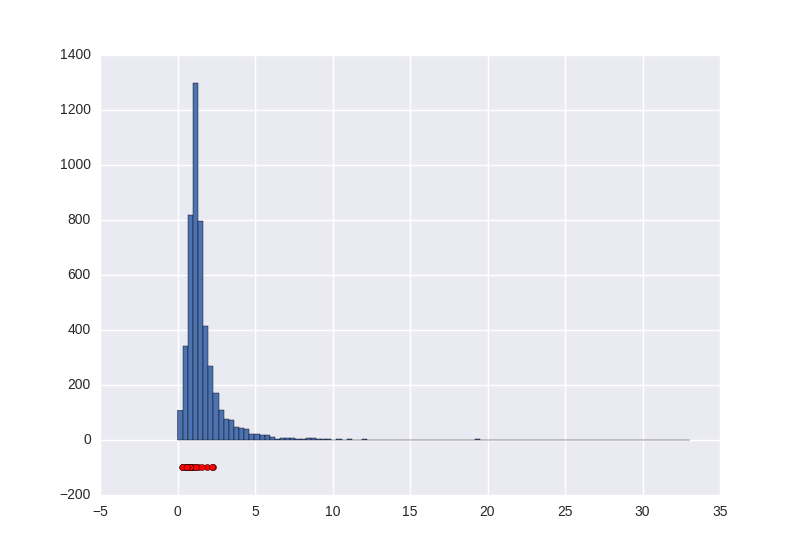
\includegraphics[width=0.8\linewidth]{r13.png}
    \caption{Liquidity, wide}
\end{figure}
\begin{figure}[h]
  \centering
  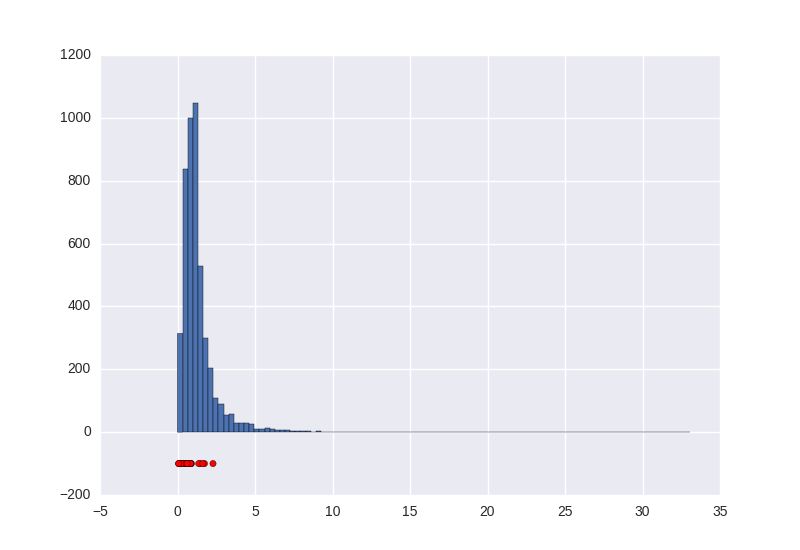
\includegraphics[width=0.8\linewidth]{r14.png}
  \caption{strict Liquidity}
\end{figure}
\begin{figure}[h]
  \centering
  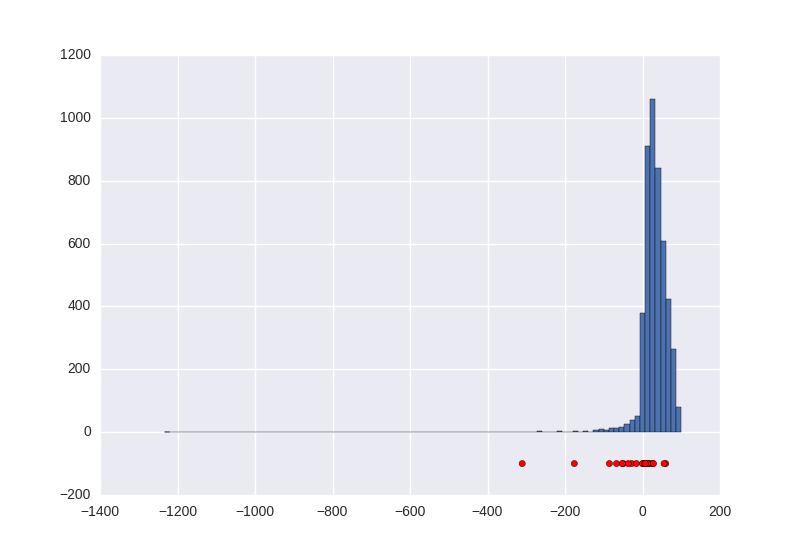
\includegraphics[width=0.8\linewidth]{r19.png}
  \caption{Net Equity / Total Assets}
\end{figure}
\clearpage

\section{Dispersion Graphics raster plots}
These scatterplots give us a sense of how we can try to capture defaulted enterprises.
\begin{figure}[h]
\centering
    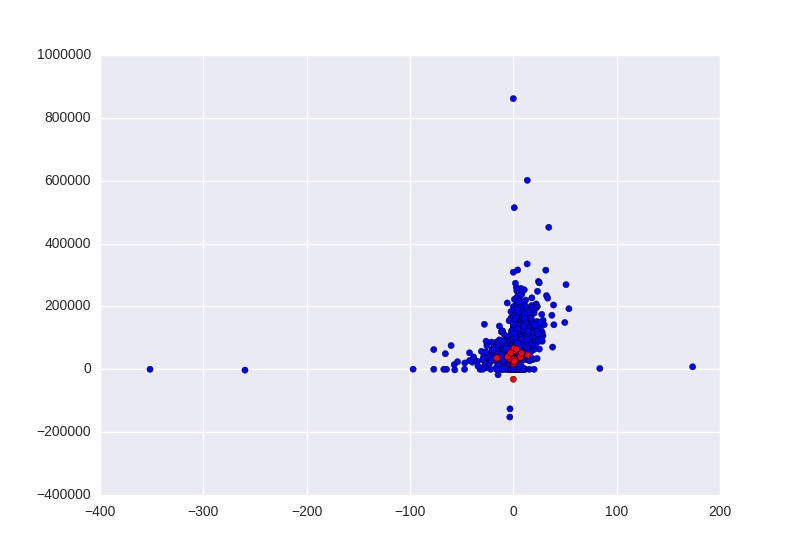
\includegraphics[width=0.8\linewidth]{cr2xr4.png}
    \caption{Net margin over sales versus added value by employee}
\end{figure}  
\begin{figure}[h]
  \centering
  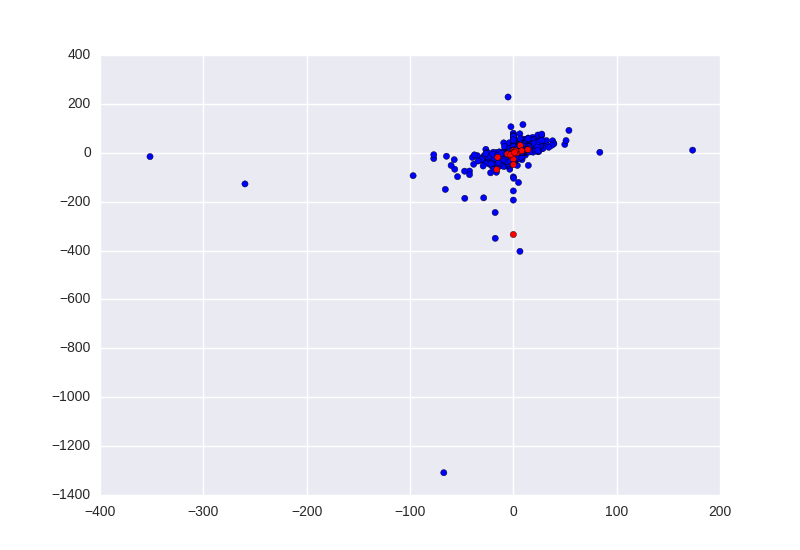
\includegraphics[width=0.8\linewidth]{cr2xr12.png}
  \caption{Sales Margin versus Net Profitability of total assets before taxed and debt charges}
\end{figure}
\begin{figure}[h]
  \centering
  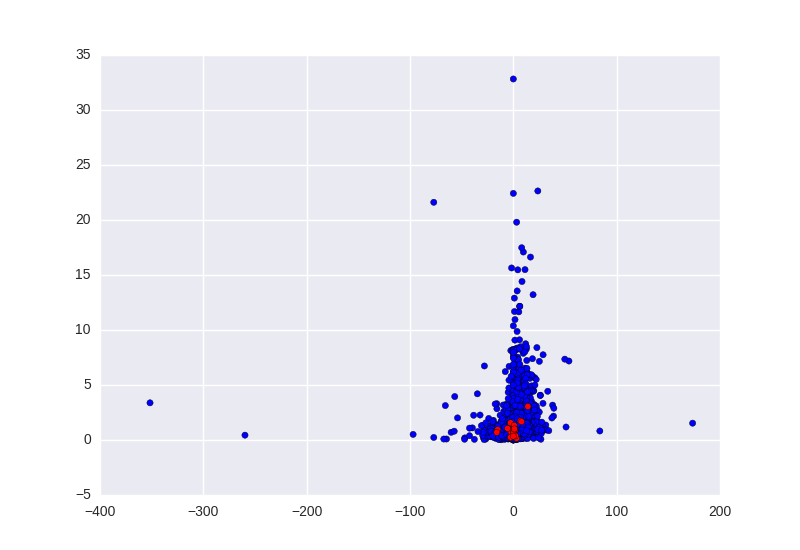
\includegraphics[width=0.8\linewidth]{cr2xr14.png}
  \caption{Net Margin over sales versus Strict liquidity}
\end{figure}
\begin{figure}[h]
  \centering
  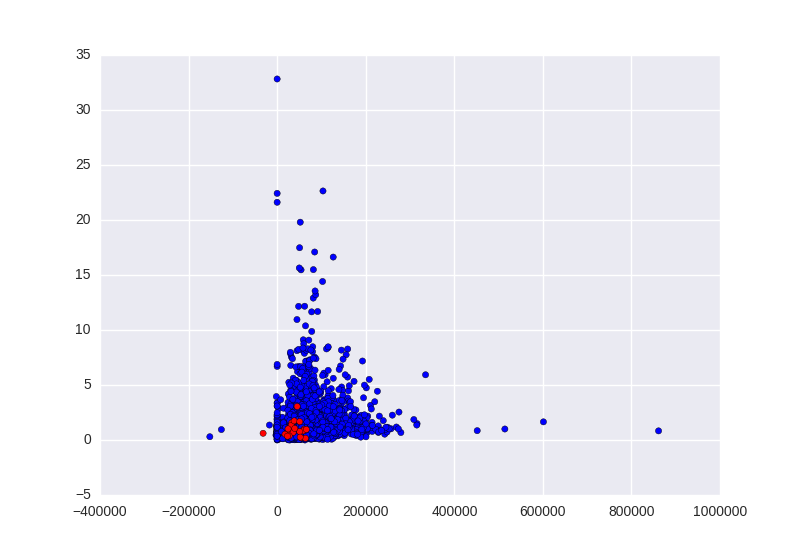
\includegraphics[width=0.8\linewidth]{cr4xr14.png}
  \caption{Added value by employee versus Strict Liquidity}
\end{figure}
\begin{figure}[h]
  \centering
  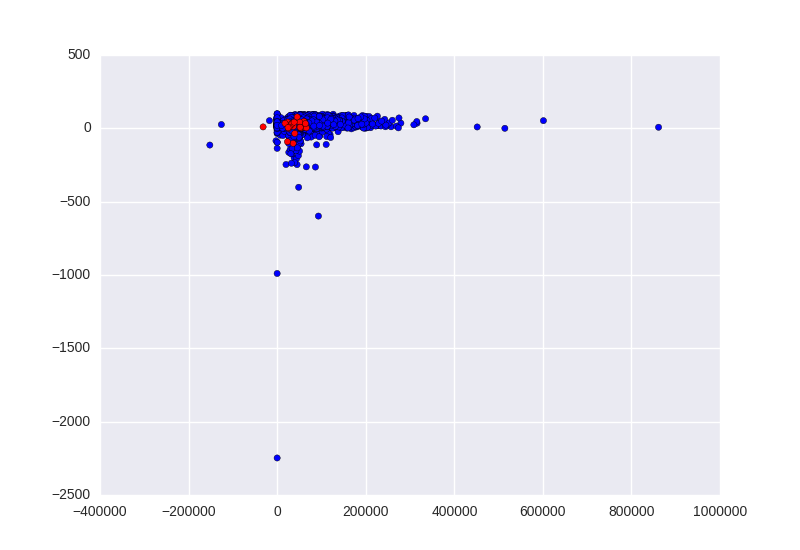
\includegraphics[width=0.8\linewidth]{cr4xr19.png}
  \caption{Added value by employee versus Net Equity over Total Assets}
\end{figure}
  \begin{figure}[h]
    \centering
    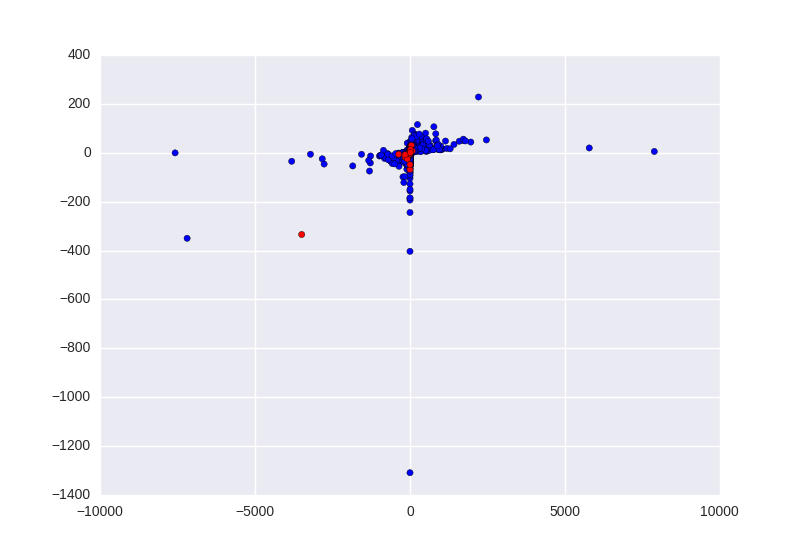
\includegraphics[width=0.8\linewidth]{cr9xr12.png}
    \caption{Net Profitability Net Profitability of total assets before taxes over debt cost}
  \end{figure}
  \begin{figure}[h]
    \centering
    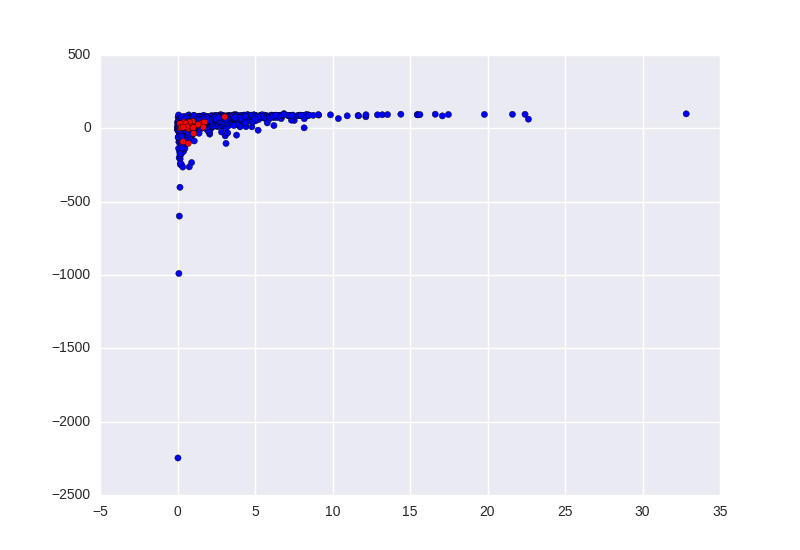
\includegraphics[width=0.8\linewidth]{cr14xr19.png}
    \caption{Strict Liquidity versus Equity over Total Assets}
  \end{figure}
\end{appendices}
\clearpage


\begin{thebibliography}{99} 
\bibitem{Altman}
E. Altman
\newblock Predicting Financial Distress of Companies: revisiting the Z-Score and Zeta Models.
\newblock {\em  New York University}

\bibitem{Bishop}
C. M. Bishop.
\newblock Pattern Recognition and Machine Learning
\newblock {\em Springer}

\bibitem{HTF}
T. Hastie, R. Tibshirani, J. Friedman
\newblock The Elements of Statistical Learning
\newblock {\em Springer}

\bibitem{ross}
S. M. Ross
\newblock Introduction to Probability Models
\newblock {\em Academc Press}

\bibitem{Thibierge}
C. Thibierge
\newblock Analyse Financière
\newblock {\em Vuibert}

\bibitem{wass}
L. Wasserman
\newblock All of Statistics
\newblock {\em Springer}
\end{thebibliography}
%----------------------------------------------------------------------------------------

\end{document}
